% cpu/overview.tex

\section{Overview}
\label{sec:cpu:Overview}

Careless reading of computer-system specification sheets might lead one
to believe that CPU performance is a footrace on a clear track, as
illustrated in Figure~\ref{fig:cpu:CPU Performance at its Best},
where the race always goes to the swiftest.

\begin{figure}[htb]
\centering
\resizebox{3in}{!}{\includegraphics{cartoons/r-2014-CPU-track-meet}}
\caption{CPU Performance at its Best}
\ContributedBy{Figure}{fig:cpu:CPU Performance at its Best}{Melissa Broussard}
\end{figure}

Although there are a few CPU-bound benchmarks that approach the ideal
shown in Figure~\ref{fig:cpu:CPU Performance at its Best},
the typical program more closely resembles an obstacle course than
a race track.
This is because the internal architecture of CPUs has changed dramatically
over the past few decades, courtesy of Moore's Law.
These changes are described in the following sections.

\subsection{Pipelined CPUs}
\label{sec:cpu:Pipelined CPUs}

\begin{figure}[tb]
\centering
\resizebox{3in}{!}{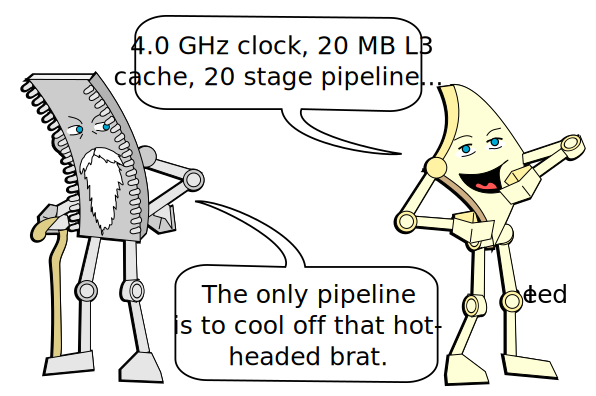
\includegraphics{cartoons/r-2014-Old-man-and-Brat}}
\caption{CPUs Old and New}
\ContributedBy{Figure}{fig:cpu:CPUs Old and New}{Melissa Broussard}
\end{figure}

In the early 1980s, the typical microprocessor fetched an instruction,
decoded it, and executed it, typically taking \emph{at least} three
clock cycles to complete one instruction before proceeding to the next.
In contrast, the CPU of the late 1990s and early 2000s will be executing
many instructions simultaneously, using a deep ``pipeline'' to control
the flow of instructions internally to the CPU.
These modern hardware features can greatly improve performance, as
illustrated by Figure~\ref{fig:cpu:CPUs Old and New}.

Achieving full performance with a CPU having a long pipeline requires
highly predictable control flow through the program.
Suitable control flow can be provided by a program that executes primarily
in tight loops, for example, arithmetic on large matrices or vectors.
The CPU can then correctly predict that the branch at the end of the loop
will be taken in almost all cases,
allowing the pipeline to be kept full and the CPU to execute at full speed.

\begin{figure}[tb]
\centering
\resizebox{3in}{!}{\includegraphics{cartoons/r-2014-branch-error}}
\caption{CPU Meets a Pipeline Flush}
\ContributedBy{Figure}{fig:cpu:CPU Meets a Pipeline Flush}{Melissa Broussard}
\end{figure}

However, branch prediction is not always so easy.
For example, consider a program with many loops, each of which iterates
a small but random number of times.
For another example, consider
an object-oriented program with many virtual objects that
can reference many different real objects, all with different implementations
for frequently invoked member functions.
In these cases, it is difficult or even
impossible for the CPU to predict where the next branch might lead.
Then either the CPU must stall waiting for execution to proceed far
enough to be certain where that branch leads, or it must guess.
Although guessing works extremely well for programs with predictable
control flow, for unpredictable branches (such as those in binary search)
the guesses will frequently be wrong.
A wrong guess can be expensive because the CPU must discard any
speculatively executed instructions following the corresponding
branch, resulting in a pipeline flush.
If pipeline flushes appear too frequently, they drastically reduce
overall performance, as fancifully depicted in
Figure~\ref{fig:cpu:CPU Meets a Pipeline Flush}.

Unfortunately, pipeline flushes are not the only hazards in the obstacle
course that modern CPUs must run.
The next section covers the hazards of referencing memory.

\subsection{Memory References}
\label{sec:cpu:Memory References}

In the 1980s, it often took less time for a microprocessor to load a value
from memory than it did to execute an instruction.
In 2006, a microprocessor might be capable of executing hundreds or even
thousands of instructions in the time required to access memory.
This disparity is due to the fact that Moore's Law has increased CPU
performance at a much greater rate than it has decreased memory latency,
in part due to the rate at which memory sizes have grown.
For example, a typical 1970s minicomputer might have 4\,KB (yes, kilobytes,
not megabytes, let alone gigabytes) of main memory, with
single-cycle access.\footnote{
	It is only fair to add that each of these single cycles
	lasted no less than 1.6 \emph{microseconds}.}
In 2008, CPU designers still can construct a 4\,KB memory with single-cycle
access, even on systems with multi-GHz clock frequencies.
And in fact they frequently do construct such memories, but they now
call them ``level-0 caches'', and they can be quite a bit bigger than 4\,KB.

\begin{figure}[htb]
\centering
\resizebox{3in}{!}{\includegraphics{cartoons/r-2014-memory-reference}}
\caption{CPU Meets a Memory Reference}
\ContributedBy{Figure}{fig:cpu:CPU Meets a Memory Reference}{Melissa Broussard}
\end{figure}

Although the large caches found on modern microprocessors can do quite
a bit to help combat memory-access latencies,
these caches require highly predictable data-access patterns to
successfully hide those latencies.
Unfortunately, common operations such as traversing a linked list
have extremely unpredictable memory-access patterns---after all,
if the pattern was predictable, us software types would not bother
with the pointers, right?
Therefore, as shown in
Figure~\ref{fig:cpu:CPU Meets a Memory Reference},
memory references often pose severe obstacles to modern CPUs.

Thus far, we have only been considering obstacles that can arise during
a given CPU's execution of single-threaded code.
Multi-threading presents additional obstacles to the CPU, as
described in the following sections.

\subsection{Atomic Operations}
\label{sec:cpu:Atomic Operations}

One such obstacle is atomic operations.
The problem here is that the whole idea of an atomic operation conflicts with
the piece-at-a-time assembly-line operation of a CPU pipeline.
To hardware designers' credit, modern CPUs use a number of extremely clever
tricks to make such operations \emph{look} atomic even though they
are in fact being executed piece-at-a-time,
with one common trick being to identify all the cachelines containing the
data to be atomically operated on,
ensure that these cachelines are owned by the CPU executing the
atomic operation, and only then proceed with the atomic operation
while ensuring that these cachelines remained owned by this CPU.
Because all the data is private to this CPU, other CPUs are unable to
interfere with the atomic operation despite the piece-at-a-time nature
of the CPU's pipeline.
Needless to say, this sort of trick can require that
the pipeline must be delayed or even flushed in order to
perform the setup operations that
permit a given atomic operation to complete correctly.

\begin{figure}[htb]
\centering
\resizebox{3in}{!}{\includegraphics{cartoons/r-2014-Atomic-reference}}
\caption{CPU Meets an Atomic Operation}
\ContributedBy{Figure}{fig:cpu:CPU Meets an Atomic Operation}{Melissa Broussard}
\end{figure}

In contrast, when executing a non-atomic operation, the CPU can load
values from cachelines as they appear and place the results in the
store buffer, without the need to wait for cacheline ownership.
Fortunately, CPU designers have focused heavily on atomic operations,
so that as of early 2014 they have greatly reduced their overhead.
Even so, the resulting effect on performance is all too often as depicted in
Figure~\ref{fig:cpu:CPU Meets an Atomic Operation}.

Unfortunately, atomic operations usually apply only to single elements
of data.
Because many parallel algorithms require that ordering constraints
be maintained between updates of multiple data elements, most CPUs
provide memory barriers.
These memory barriers also serve as performance-sapping obstacles,
as described in the next section.

\QuickQuiz{}
	What types of machines would allow atomic operations on
	multiple data elements?
\QuickQuizAnswer{
	One answer to this question is that it is often possible to
	pack multiple elements of data into a single machine word,
	which can then be manipulated atomically.

	A more trendy answer would be machines supporting transactional
	memory~\cite{DBLomet1977SIGSOFT}.
	As of early 2014, several mainstream systems provide limited
	hardware transactional memory implementations, which is covered
	in more detail in
	Section~\ref{sec:future:Hardware Transactional Memory}.
	The jury is still out on the applicability of software transactional
	memory~\cite{McKenney2007PLOSTM,DonaldEPorter2007TRANSACT,
	ChistopherJRossbach2007a,CalinCascaval2008tmtoy,
	AleksandarDragovejic2011STMnotToy,AlexanderMatveev2012PessimisticTM}.
	Additional information on software transactional memory may be
	found in
	Section~\ref{sec:future:Transactional Memory}.
} \QuickQuizEnd

\subsection{Memory Barriers}
\label{sec:cpu:Memory Barriers}

Memory barriers will be considered in more detail in
Chapter~\ref{chp:Advanced Synchronization: Memory Ordering} and
Appendix~\ref{chp:app:whymb:Why Memory Barriers?}.
In the meantime, consider the following simple lock-based critical
section:

\begin{VerbatimN}
spin_lock(&mylock);
a = a + 1;
spin_unlock(&mylock);
\end{VerbatimN}

\begin{figure}[tb]
\centering
\resizebox{3in}{!}{\includegraphics{cartoons/r-2014-Memory-barrier}}
\caption{CPU Meets a Memory Barrier}
\ContributedBy{Figure}{fig:cpu:CPU Meets a Memory Barrier}{Melissa Broussard}
\end{figure}

If the CPU were not constrained to execute these statements in the
order shown, the effect would be that the variable ``a'' would be
incremented without the protection of ``mylock'', which would certainly
defeat the purpose of acquiring it.
To prevent such destructive reordering, locking primitives contain
either explicit or implicit memory barriers.
Because the whole purpose of these memory barriers is to prevent reorderings
that the CPU would otherwise undertake in order to increase performance,
memory barriers almost always reduce performance, as depicted in
Figure~\ref{fig:cpu:CPU Meets a Memory Barrier}.

As with atomic operations, CPU designers have been working hard to
reduce memory-barrier overhead, and have made substantial progress.

\subsection{Cache Misses}
\label{sec:cpu:Cache Misses}

\begin{figure}[tb]
\centering
\resizebox{3in}{!}{\includegraphics{cartoons/r-2014-CPU-track-meet-cache-miss-toll-booth}}
\caption{CPU Meets a Cache Miss}
\ContributedBy{Figure}{fig:cpu:CPU Meets a Cache Miss}{Melissa Broussard}
\end{figure}

An additional multi-threading obstacle to CPU performance is
the ``cache miss''.
As noted earlier, modern CPUs sport large caches in order to reduce the
performance penalty that would otherwise be incurred due to high memory
latencies.
However, these caches are actually counter-productive for variables that
are frequently shared among CPUs.
This is because when a given CPU wishes to modify the variable, it is
most likely the case that some other CPU has modified it recently.
In this case, the variable will be in that other CPU's cache, but not
in this CPU's cache, which will therefore incur an expensive cache miss
(see Section~\ref{sec:app:whymb:Cache Structure} for more detail).
Such cache misses form a major obstacle to CPU performance, as shown
in Figure~\ref{fig:cpu:CPU Meets a Cache Miss}.

\QuickQuiz{}
	So have CPU designers also greatly reduced the overhead of
	cache misses?
\QuickQuizAnswer{
	Unfortunately, not so much.
	There has been some reduction given constant numbers of CPUs,
	but the finite speed of light and the atomic nature of
	matter limits their ability to reduce cache-miss overhead
	for larger systems.
	Section~\ref{sec:cpu:Hardware Free Lunch?}
	discusses some possible avenues for possible future progress.
} \QuickQuizEnd

\subsection{I/O Operations}
\label{sec:cpu:I/O Operations}

\begin{figure}[tb]
\centering
\resizebox{3in}{!}{\includegraphics{cartoons/r-2014-CPU-track-meet-phone-booth}}
\caption{CPU Waits for I/O Completion}
\ContributedBy{Figure}{fig:cpu:CPU Waits for I/O Completion}{Melissa Broussard}
\end{figure}

A cache miss can be thought of as a CPU-to-CPU I/O operation, and as
such is one of the cheapest I/O operations available.
I/O operations involving networking, mass storage, or (worse yet) human
beings pose much greater obstacles than the internal obstacles called
out in the prior sections,
as illustrated by
Figure~\ref{fig:cpu:CPU Waits for I/O Completion}.

This is one of the differences between shared-memory and distributed-system
parallelism: shared-memory parallel programs must normally deal with no
obstacle worse than a cache miss, while a distributed parallel program
will typically incur the larger network communication latencies.
In both cases, the relevant latencies can be thought of as a cost of
communication---a cost that would be absent in a sequential program.
Therefore, the ratio between the overhead of the communication to
that of the actual work being performed is a key design parameter.
A major goal of parallel hardware design is to reduce this ratio as
needed to achieve the relevant performance and scalability goals.
In turn, as will be seen in
Chapter~\ref{cha:Partitioning and Synchronization Design},
a major goal of parallel software design is to reduce the
frequency of expensive operations like communications cache misses.

Of course, it is one thing to say that a given operation is an obstacle,
and quite another to show that the operation is a \emph{significant}
obstacle.
This distinction is discussed in the following sections.
